\documentclass[a4paper,10.5pt]{article}
\usepackage{hieroglf} % 添加古埃及象形文字
\usepackage{pifont} % 添加 Dingbat

\usepackage[top=1in,bottom=1in,left=1in,right=1in]{geometry} % 用于设置页面布局
\usepackage{xeCJK} % 用于使用本地字体
\usepackage[super, square, sort&compress]{natbib} % 处理参考文献
\usepackage{titlesec, titletoc} % 设置章节标题及页眉页脚
%\usepackage{xCJKnumb} % 中英文数字转换
\usepackage{amssymb}
\usepackage{amsmath} % 在公式中用\text{文本}输入中文
\usepackage{diagbox}
\usepackage{multirow} % 表格中使用多行
\usepackage{booktabs} % 表格中使用\toprule等命令
\usepackage{rotating} % 使用sidewaystable环境旋转表格
\usepackage{tabularx}
\usepackage{graphicx} % 处理图片
\usepackage{footnote} % 增强的脚注功能,可添加表格脚注
\usepackage{threeparttable} % 添加真正的表格脚注,示例见README
\usepackage{hyperref} % 添加pdf书签

\usepackage{tikz}
\usetikzlibrary{shapes,arrows,shadows}

% 字体设置
\setmainfont{Times New Roman}
\setsansfont[Scale=MatchLowercase,Mapping=tex-text]{PT Sans}
\setmonofont[Scale=MatchLowercase]{PT Mono}
\setCJKmainfont[ItalicFont={Kaiti SC}, BoldFont={Heiti SC}]{Songti SC}
\setCJKsansfont{Heiti SC}
\setCJKmonofont{Songti SC}
% \setCJKmainfont[BoldFont={FZXiaoBiaoSong-B05S}]{Songti SC}
% \setCJKfamilyfont{kai}[BoldFont=Heiti SC]{Kaiti SC}
% \setCJKfamilyfont{song}[BoldFont=Heiti SC]{Songti SC}
% \setCJKfamilyfont{hei}[BoldFont=Heiti SC]{Heiti SC}
% \setCJKfamilyfont{fsong}[BoldFont=Heiti SC]{Songti SC}
% \newcommand{\kai}[1]{{\CJKfamily{kai}#1}}
% \newcommand{\hei}[1]{{\CJKfamily{hei}#1}}
% \setromanfont[Mapping=tex-text]{TeXGyrePagella}
% \setsansfont[Scale=MatchLowercase,Mapping=tex-text]{TeXGyrePagella}
% \setmonofont[Scale=MatchLowercase]{Courier New}
%%设置常用中文字号,方便调用
\newcommand{\erhao}{\fontsize{22pt}{\baselineskip}\selectfont}
\newcommand{\xiaoerhao}{\fontsize{18pt}{\baselineskip}\selectfont}
\newcommand{\sanhao}{\fontsize{16pt}{\baselineskip}\selectfont}
\newcommand{\xiaosanhao}{\fontsize{15pt}{\baselineskip}\selectfont}
\newcommand{\sihao}{\fontsize{14pt}{\baselineskip}\selectfont}
\newcommand{\xiaosihao}{\fontsize{12pt}{\baselineskip}\selectfont}
\newcommand{\wuhao}{\fontsize{10.5pt}{\baselineskip}\selectfont}
\newcommand{\xiaowuhao}{\fontsize{9pt}{\baselineskip}\selectfont}
\newcommand{\liuhao}{\fontsize{7.5pt}{\baselineskip}\selectfont}

% 章节标题显示方式及页眉页脚设置
% \item xCJKnumb是自己额外安装的包
% \item titleformat命令定义标题的形式
% \item titlespacing定义标题距左、上、下的距离
\titleformat{\section}{\raggedright\large\bfseries}{\thesection}{1em}{}
\titleformat{\subsection}{\raggedright\normalsize\bfseries}{\thesubsection}{1em}{}
\titlespacing{\section}{0pt}{*0}{*2}
\titlespacing{\subsection}{0pt}{*0}{*1}
% 由于默认的2em缩进不够,所以我手动调整了,但是在windows下似乎2.2就差不多了,或者是article中没有这个问题
\setlength{\parindent}{2.2em}

% 设置表格标题前后间距
\setlength{\abovecaptionskip}{0pt}
\setlength{\belowcaptionskip}{0pt}

\renewcommand{\refname}{\bfseries{参~考~文~献}} %将Reference改为参考文献(用于 article)
% \renewcommand{\bibname}{参~考~文~献} %将bibiography改为参考文献(用于 book)
\renewcommand{\baselinestretch}{1.38} %设置行间距
\renewcommand{\figurename}{\small\ttfamily 图}
\renewcommand{\tablename}{\small\ttfamily 表}


\newcommand{\specialcell}[2][c]{%
  \begin{tabular}[#1]{@{}c@{}}#2\end{tabular}}

\pmhgfamily

\title{异星杂谭}
\author{苑明理}
\date{2016年2月}

\begin{document}

\maketitle{}


\begin{figure}[ht]
\centering
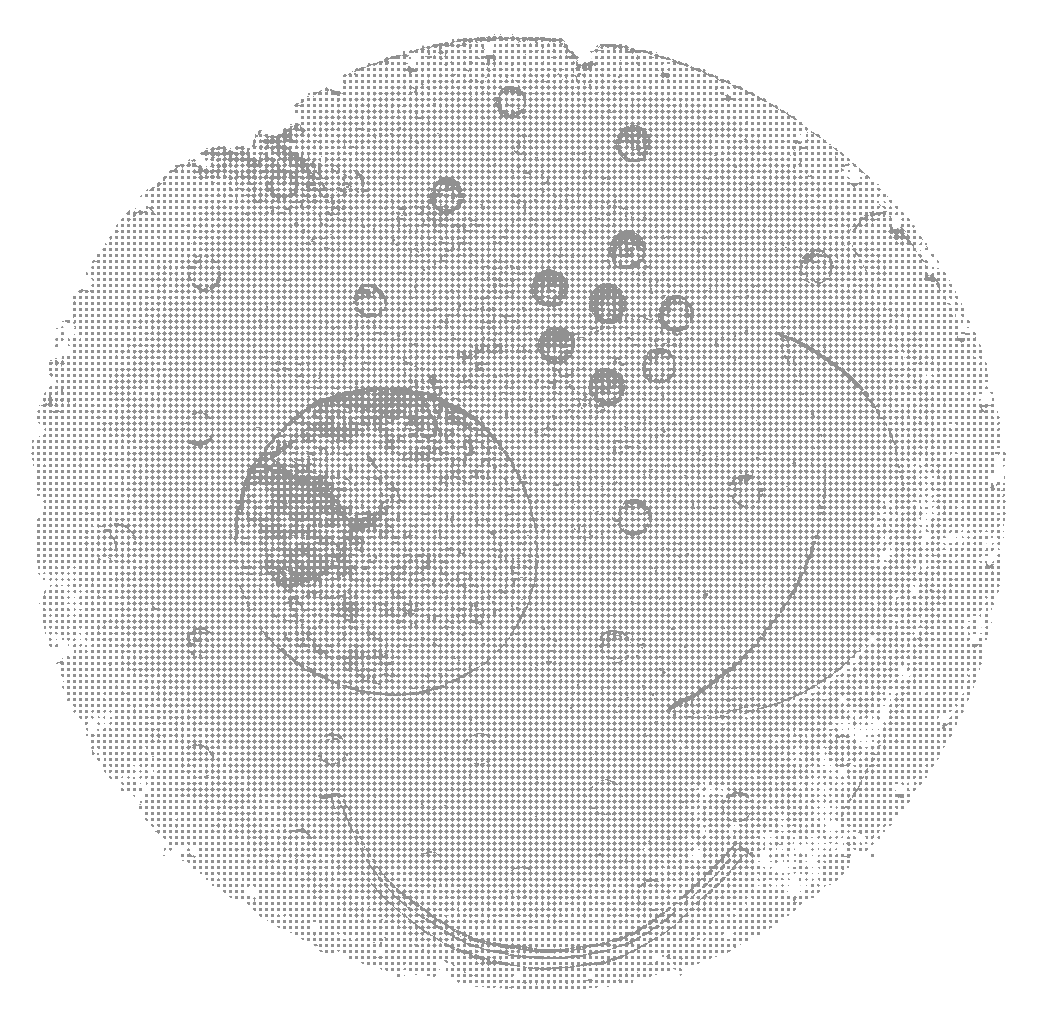
\includegraphics[width=4.5in]{images/0_00-Cover.png}
\end{figure}


\newpage
\renewcommand\contentsname{目录}
\setcounter{tocdepth}{2}
\tableofcontents

\newpage

\section{序言}

幼时夏夜,在屋顶乘凉,仰望壮丽的星空,时而会有一些遐想:在某个闪亮的星星附近,是否也有另一个“我”,同样在仰望星空,同样在发问?
后来读到 Ted Chiang 的《你一生的故事》,深为外星异质文化带来的观念冲击而着迷。为什么呢?因为人们可以通过不同来重新审视自己。

我们常常藏身于观念的硬壳里,很多观念创建已久,已经成为我们每个人思考的一部分;当我们说到它,仅仅一个熟知的词汇脱口而出,压根没想它真正的意义。
当重新尝试用观念创造者的角度来思考时,我们才恍然发现一个个想法的背后,对它们的思考并不是那么简单。不同会促使我们反省僵化的思维。

古时,庄子作的一篇篇寓言,扬雄写出《太玄》与《法言》,这些著作或许有作者的深意。今人即使不认同这些背后的想法,但也不得不惊叹古人各种不同的瑰奇想象。
想象可以通过小说来表达,却重在情节而失之知识的严谨;知识可以通过严谨的论文来表述,可缺少了情趣与浪漫。

那么这本小书想达成什么呢?仅仅是想为成长中的青少年,开启一扇可以望见星空的窗,去感受外面无限的宇宙。这是笔者在写这本书时想到的,故以此为序。

\newpage

\section{人类对宇宙的认识之路}

\subsection{远古的探寻}

自古以来,天空中的日、月、星辰引发了人们无尽的想象和探究。1999年人们在德国发现了内布拉星象盘,它是公元前16世纪青铜时代的器物。
在这个铜盘之上同时出现有太阳、月亮和星辰。根据一种解释,该盘上太阳和月亮之间的那团七星,是著名的金牛座“七姐妹”—昴宿星团。
内布拉星象盘艺术式地表现了人们对宇宙的思考与追寻。

\begin{figure}[ht]
\centering
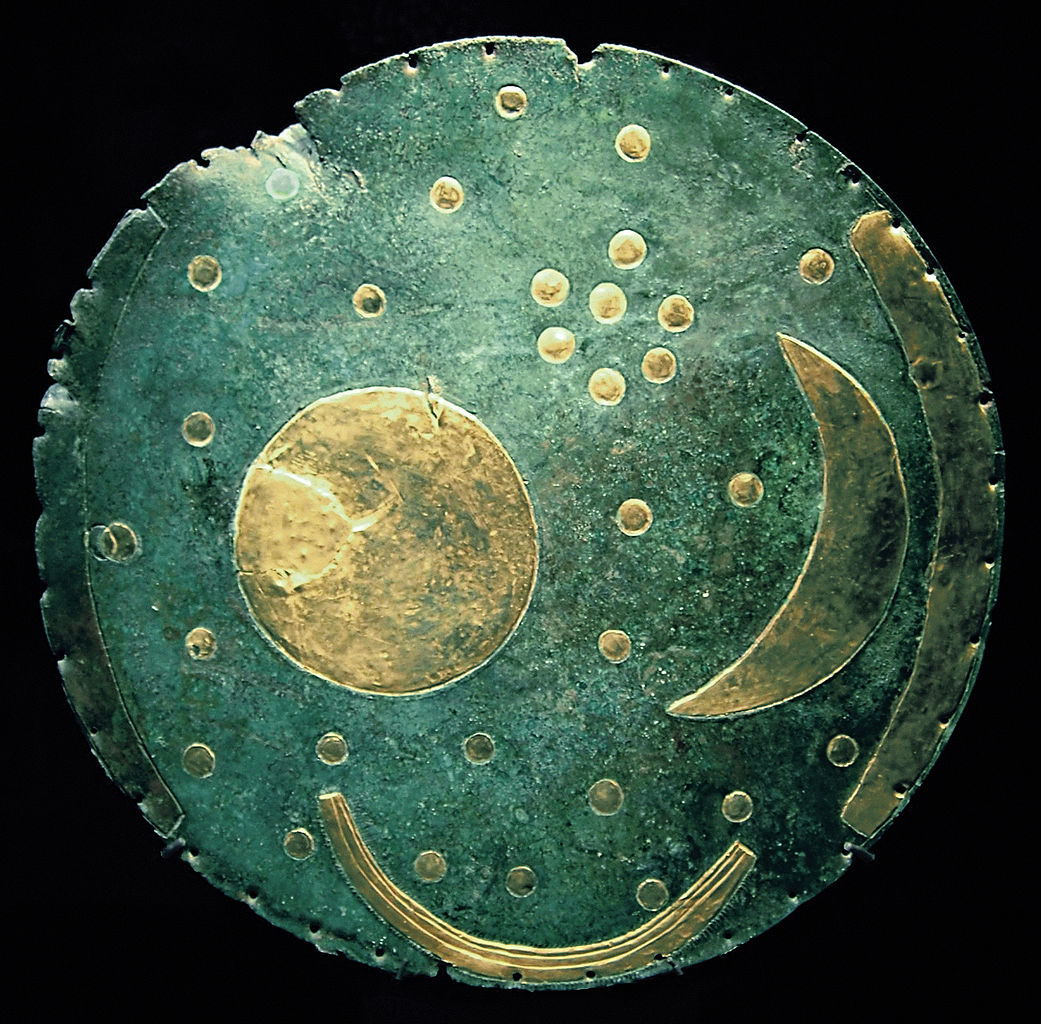
\includegraphics[width=2.5in]{images/1_01-Nebra_sky_disk.jpg}
\caption{内布拉星象盘(图片来自于维基共享资源计划)}
\end{figure}

然而人类对宇宙的追寻并不只停留在艺术式的表现,更在于能够精确预测天文现象。根据一种假说,建于公元前两、三千多年前的英国巨石阵
可以用来预测日月的位置和日食的发生。预测方法是使用巨石阵内 56 个 Aubrey 洞来实现的,它的原理是基于用公分子 56 来近似表达三个天文周期。

\begin{figure}[ht]
\centering
\includegraphics[width=4.5in]{images/1_00-Stonehenge.jpg}
\caption{巨石阵(图片来自于维基共享资源计划)}
\end{figure}

\begin{table}[tbhp]
\centering
\begin{tabular}{|c|c|c|}
\hline
天文现象 & 周期 & 近似周期 \\
\hline
太阳的运行周期 & 365.26 天 & $ 56 \times \frac{13}{2} $ \\
\hline
月球的运行周期 & 27.32 天 & $ 56 \times \frac{1}{2} $ \\
\hline
沙罗周期 & 18.61 年 & $ 56 \times \frac{1}{3} $ \\
\hline
\end{tabular}
\caption{基于 56 的日食预测原理}
\end{table}

\newpage

\subsection{文明时代}

尽管希腊人已经发展了多种不同的宇宙理论,但在古代很长时间里大多数人认为“地球是宇宙所有运动的中心”。这个命题赋予了地球无比特殊的地位。然而即便是在中世纪也有人对此产生异议。

Nicole Oresme(132x? – 1382)是欧洲中世纪晚期的哲学家,他在神学著作中表达了上帝之下的众多不同世界的可能。

\begin{figure}[ht]
\centering
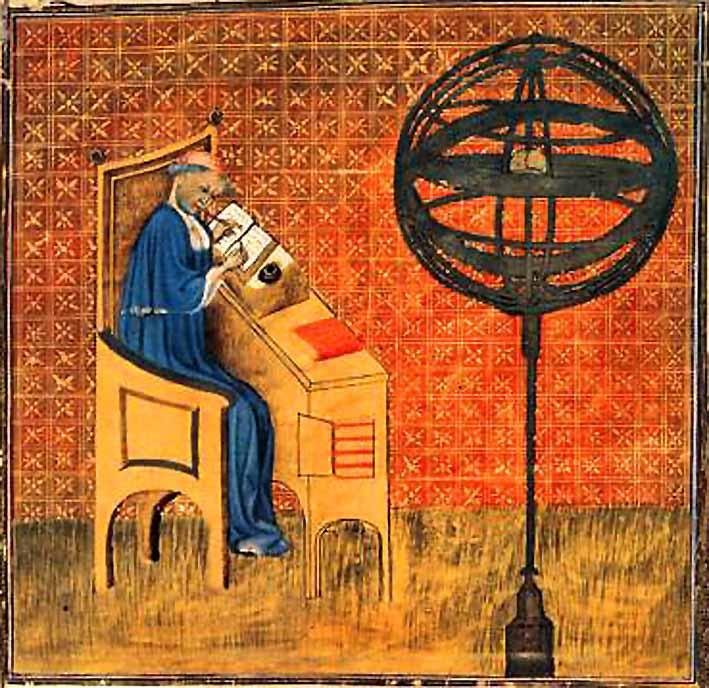
\includegraphics[width=1.5in]{images/1_02-Oresme.jpg}
\caption{Nicole Oresme(图片来自于维基共享资源计划)}
\end{figure}

\begin{figure}[ht]
\centering
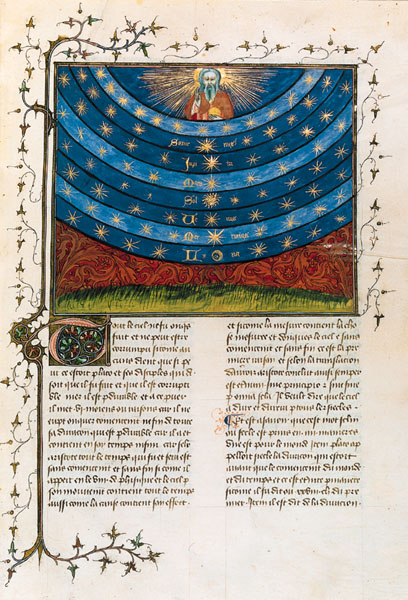
\includegraphics[width=1.5in]{images/1_03-Oresme_Spheres.jpg}
\caption{Nicole Oresme(图片来自于维基共享资源计划)}
\end{figure}

稍晚一些的 Nicholas of Cusa  (1401 – 1464) 也表达了类似的观点。

\begin{figure}[ht]
\centering
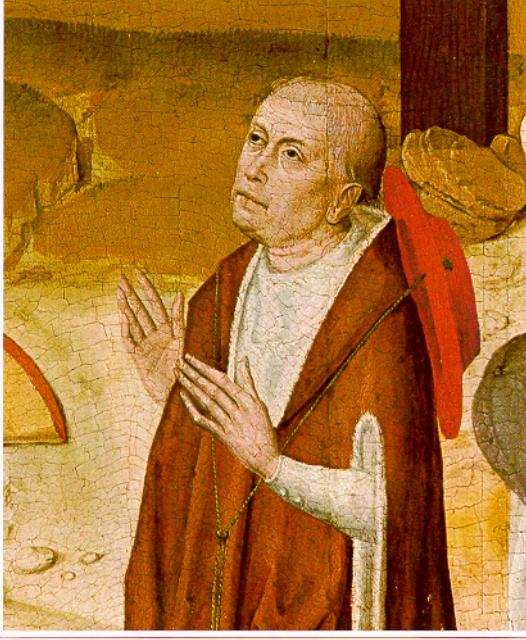
\includegraphics[width=1.5in]{images/1_04-Nicholas_of_Cusa.jpg}
\caption{Nicholas of Cusa(图片来自于维基共享资源计划)}
\end{figure}

\newpage

\subsection{文艺复兴}

其后欧洲进入文艺复兴,人才辈出。

Nicolaus Copernicus (1473 - 1543)

\begin{figure}[ht]
\centering
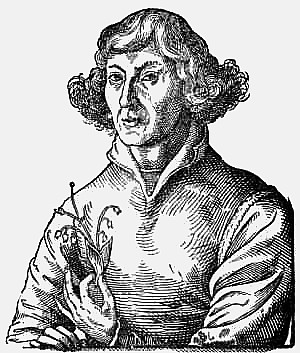
\includegraphics[width=1.5in]{images/1_05-Mikolaj_Kopernik.jpg}
\caption{哥白尼(图片来自于维基共享资源计划)}
\end{figure}

\begin{figure}[ht]
\centering
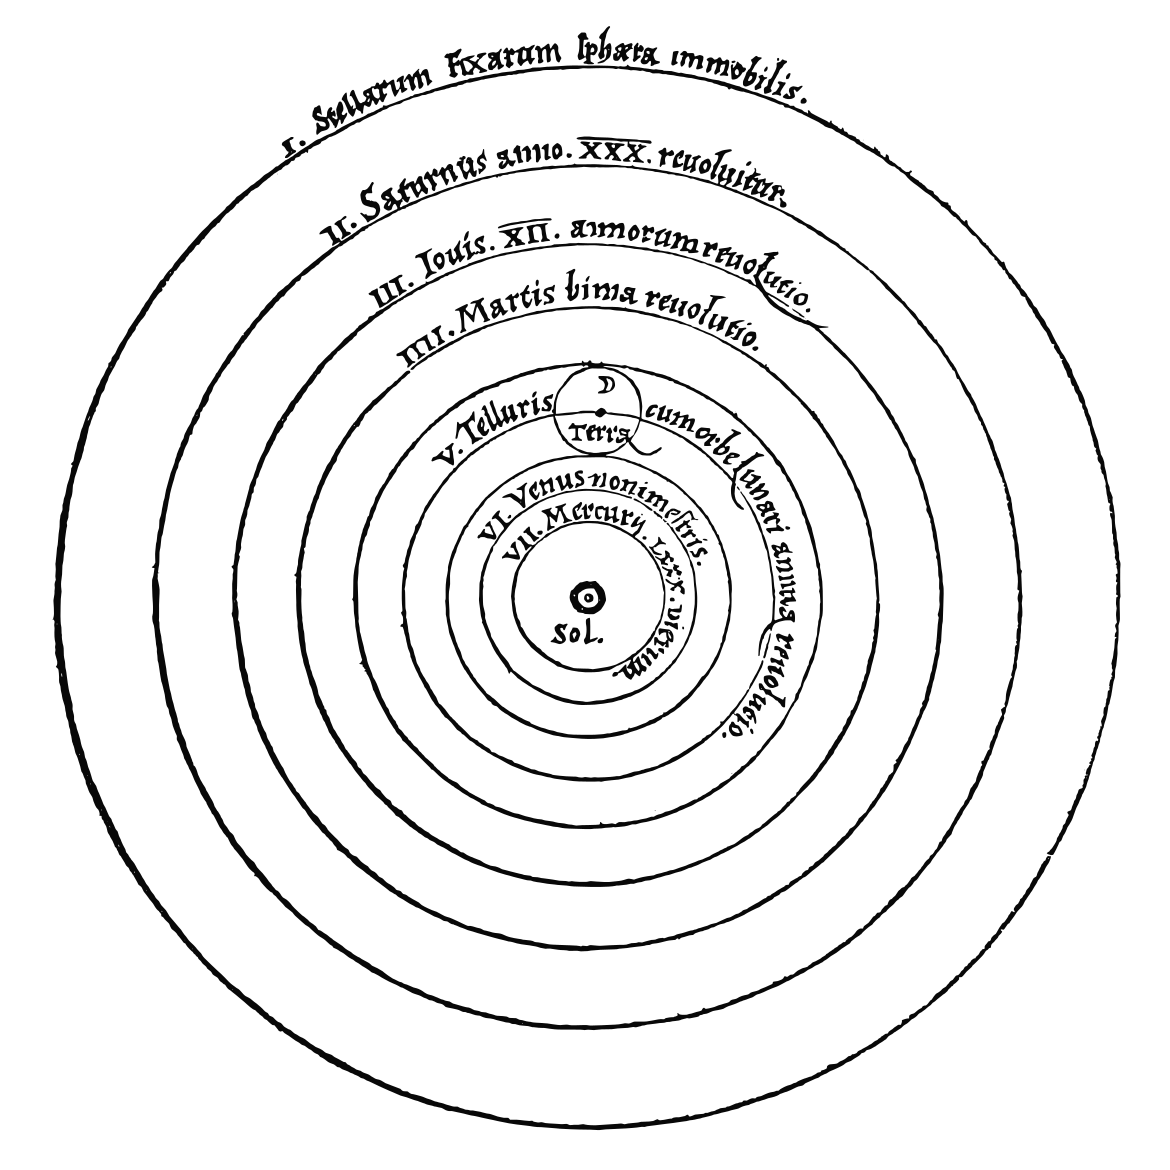
\includegraphics[width=1.5in]{images/1_06-Copernican_heliocentrism_theory_diagram.png}
\caption{《天体运行论》(图片来自于维基共享资源计划)}
\end{figure}

哥白尼在1543年去世之前,发表了著名的《天体运行论》,提出日心说,在《天体运行论》发表之后的几十年里,哥白尼的观点在欧洲不断传播。

Giordano Bruno (1548 – 1600)

布鲁诺因为他更为大胆的观点而付出了生命的代价。他认为宇宙无限,太阳是和其他恒星一样,所有恒星地位平等。

如今的罗马,在当年火刑的地点,伫立着一座布鲁诺的雕像。

\begin{figure}[ht]
\centering
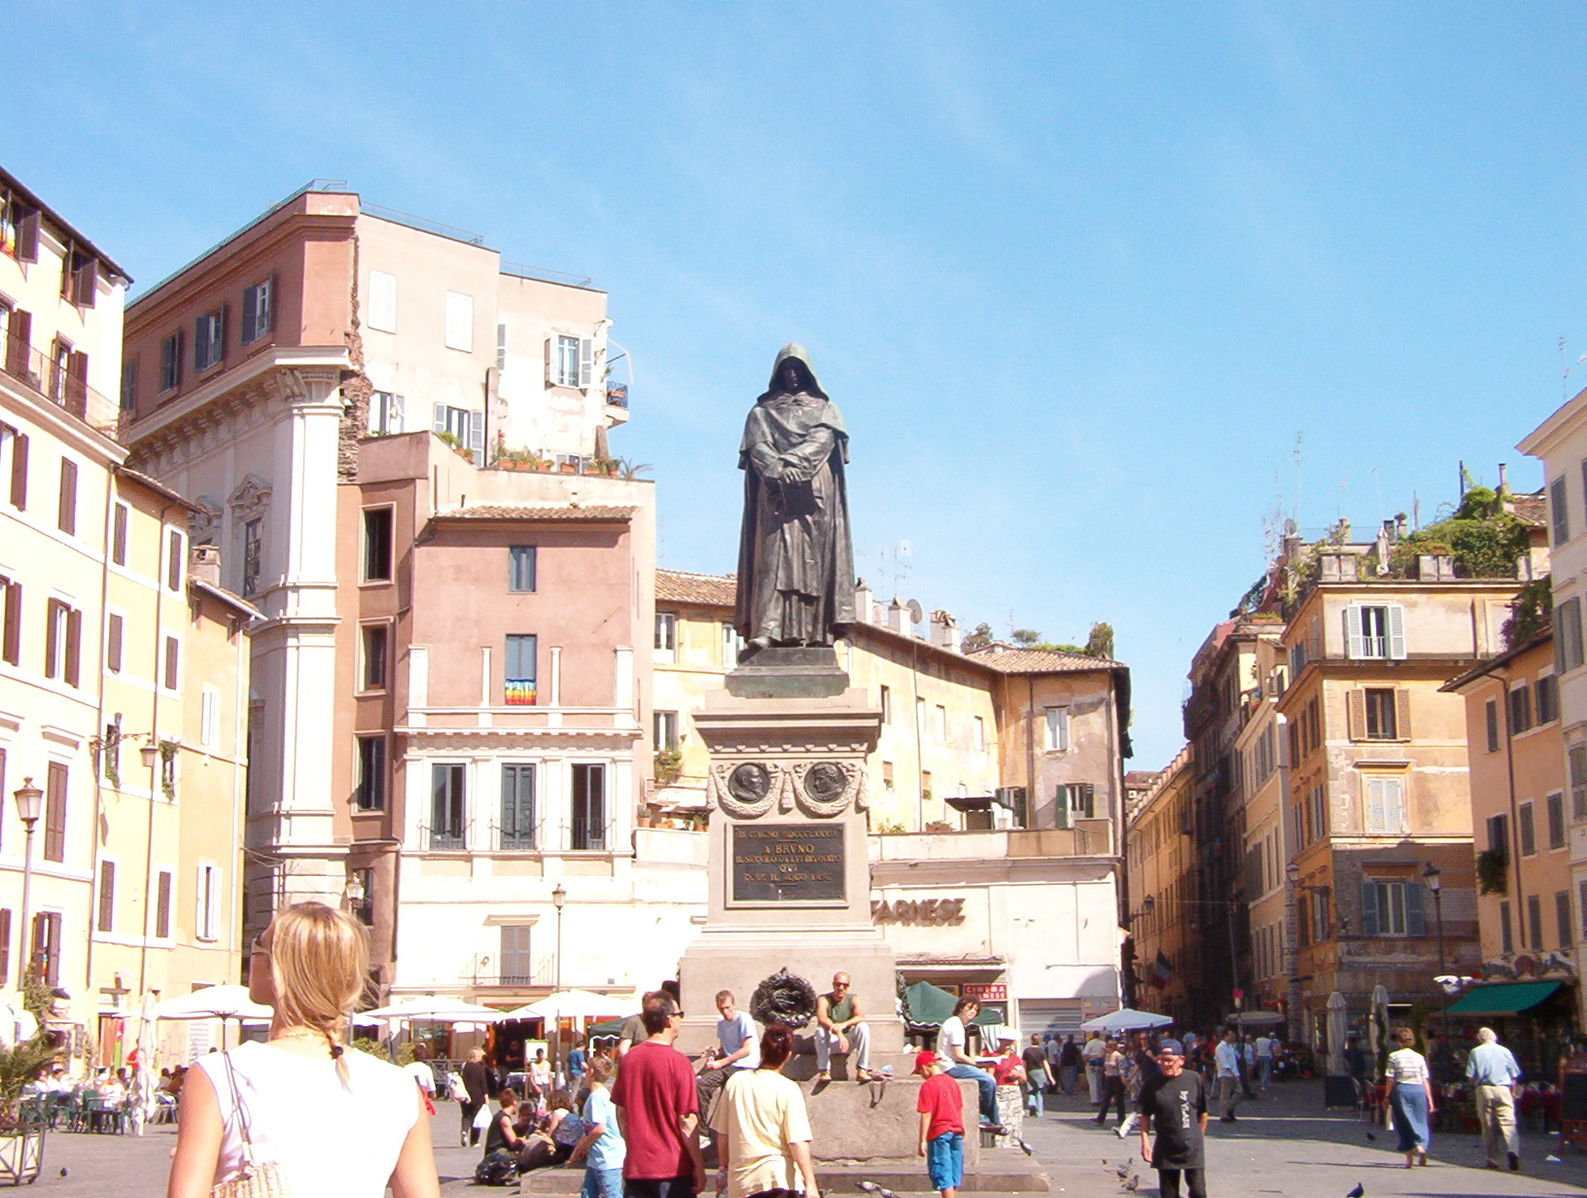
\includegraphics[width=1.5in]{images/1_07-Brunostatue.jpg}
\caption{布鲁诺像(图片来自于维基共享资源计划)}
\end{figure}

然而,在这些早期的日心说支持者中,最有贡献的是第谷。

\begin{figure}[ht]
\centering
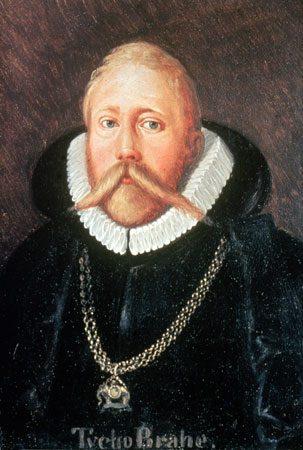
\includegraphics[width=1.5in]{images/1_08-Tycho_Brahe.jpg}
\caption{第谷(图片来自于维基共享资源计划)}
\end{figure}

Tycho Brahe (1546 – 1601)

第谷在天文学上的贡献,除了他的第谷体系之外,他还在汶岛(Hven Island)建立了天文台,从事大规模的天文观测。第谷的观测材料为他的学生开普勒的工作开辟了道路。

\begin{figure}[ht]
\centering
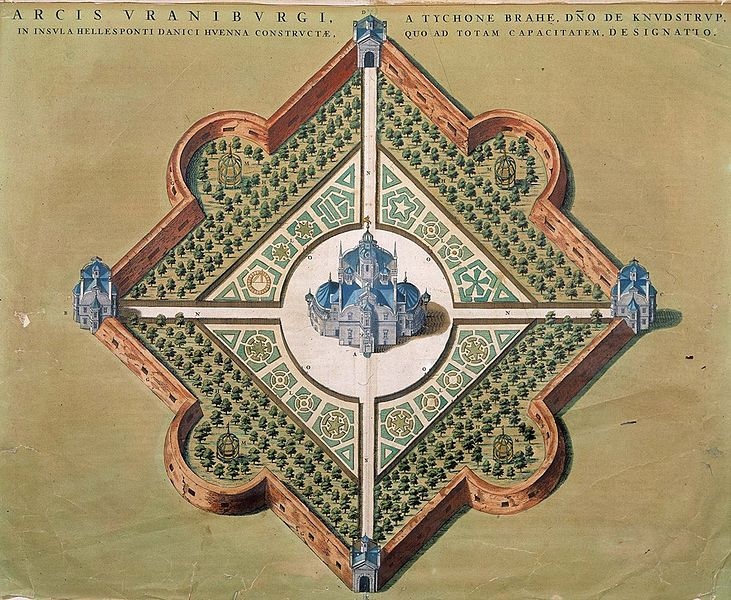
\includegraphics[width=1.5in]{images/1_09-Uraniborgskiss.jpg}
\caption{第谷建立的天文台(图片来自于维基共享资源计划)}
\end{figure}

\newpage

\subsection{近现代}

对自然深度的认识之路

开普勒建立了行星运动的三定律,开启了星体运动的数学描述之路。牛顿更进一步,发现万有引力的精确数学描述;在此基础上,拉格朗日、拉普拉斯、高斯、庞加莱建立了庞大的天体力学体系。物理学的革命:量子理论、相对论

对自然丰富的认识之路

威廉·赫歇尔(William Herschel)发现了天王星,同时他还对银河系形状建立了初步的认识。贝塞尔(Friedrich Bessel)第一次利用视差确定了太阳系到恒星天鵝座61的距离。

通过“沙普利-柯蒂斯之争”,人类确立了仙女座大星系的河外星系地位。

哈勃更利用造父变星确认河外星系的普遍存在。他还发现了河外星系的红移与距离的关系,也就是哈勃定律,为宇宙大爆炸理论提供了支持。宇宙微波背景噪音的观测。

系外行星

\newpage

\section{运动的星体}

\subsection{运动方程}

下面我们先从星体的动力学方程开始讨论。我们指定两颗恒星的下标分别是1、2,行星的下标为,于是三个星体的质量分别是$m_1$、$m_2$、$m_3$,
位置分别是矢量 $\mathbf{x_1}$、$\mathbf{x_2}$、$\mathbf{x_3}$;因为行星质量 $m_3$ 远小于两个恒星的质量,可建立如下限定性三体问题的运动方程:

$$
\begin{cases}
\ddot{\mathbf{x_1}} = Gm_2r_{12}^{-2} \mathbf{e_{12}}\\
\ddot{\mathbf{x_2}} = Gm_1r_{21}^{-2} \mathbf{e_{21}}\\
\ddot{\mathbf{x_3}} = Gm_1r_{31}^{-2} \mathbf{e_{31}} + Gm_2r_{32}^{-2} \mathbf{e_{32}}
\end{cases}
$$

其中$r_{ij}$ 为星体 i 和 j 之间的距离,$\mathbf{e_{ij}}$ 为星体 i 和 j 之间的单位方向矢量。

\subsection{方程的解算}

\subsection{天球系统}

\subsection{宜居性}

我们以液态水的稳定存在作为行星的宜居条件,可以做如下最为粗略的估计。假设母星为黑体且表面温度分别为 $T_1$ 和 $T_2$ ,母星的半径分别为 $R_1$ 和 $R_2$,瓦克星的行星反照率为 $\alpha$,半径为 $R_3$ ,视瓦克星为黑体且表面温度为 $T_3$  ,可以建立如下方程:

$$\left ( 1 - \alpha \right ) \left(  \frac{4 \pi R_1^2 \sigma T_1^4} {4 \pi r_{13}^2} + \frac{4 \pi R_2^2 \sigma T_2^4} {4 \pi r_{23}^2} \right ) \pi R_3^2= 4 \pi R_3^2 \sigma T_3^4$$

化简即得:

$$T_3 = \left[ \frac{1}{4} \left( 1 - \alpha \right ) \left( \frac{R_1^2}{r_{13}^2} T_1^4 + \frac{R_2^2}{r_{23}^2} T_2^4 \right ) \right ]^{\frac{1}{4}}$$

对地球而言,$\alpha$ 取值在 0.3 附近。

考虑到大气层的温室效应,我们只要令 $T_3$ 保持在 0 附近即可。

虽然这里宜居条件的估计涉及行星表面的物理机制,但最终化简的公式里,只保留了一些纯几何量的简单对比。所以,我们仍然把宜居问题的粗略估计纳入到恒星系建模的范围里。

\subsection{四方位}

方位感是人类内在生物机制。可是空间上的秩序并非空间自有的属性,是人类叠加到物理世界上的。可以说四方位、地名的概念是人类发明的最早的增强现实(Augmented Reality)的技术了。

从苏州地区的夜间卫星地图中的灯光可以看出,城市的街道格局是沿着东、西、南、北四个方向展开的。这其中的原因是因为在温带房子南北布局才能充分获得阳光。

\begin{figure}[ht]
\centering
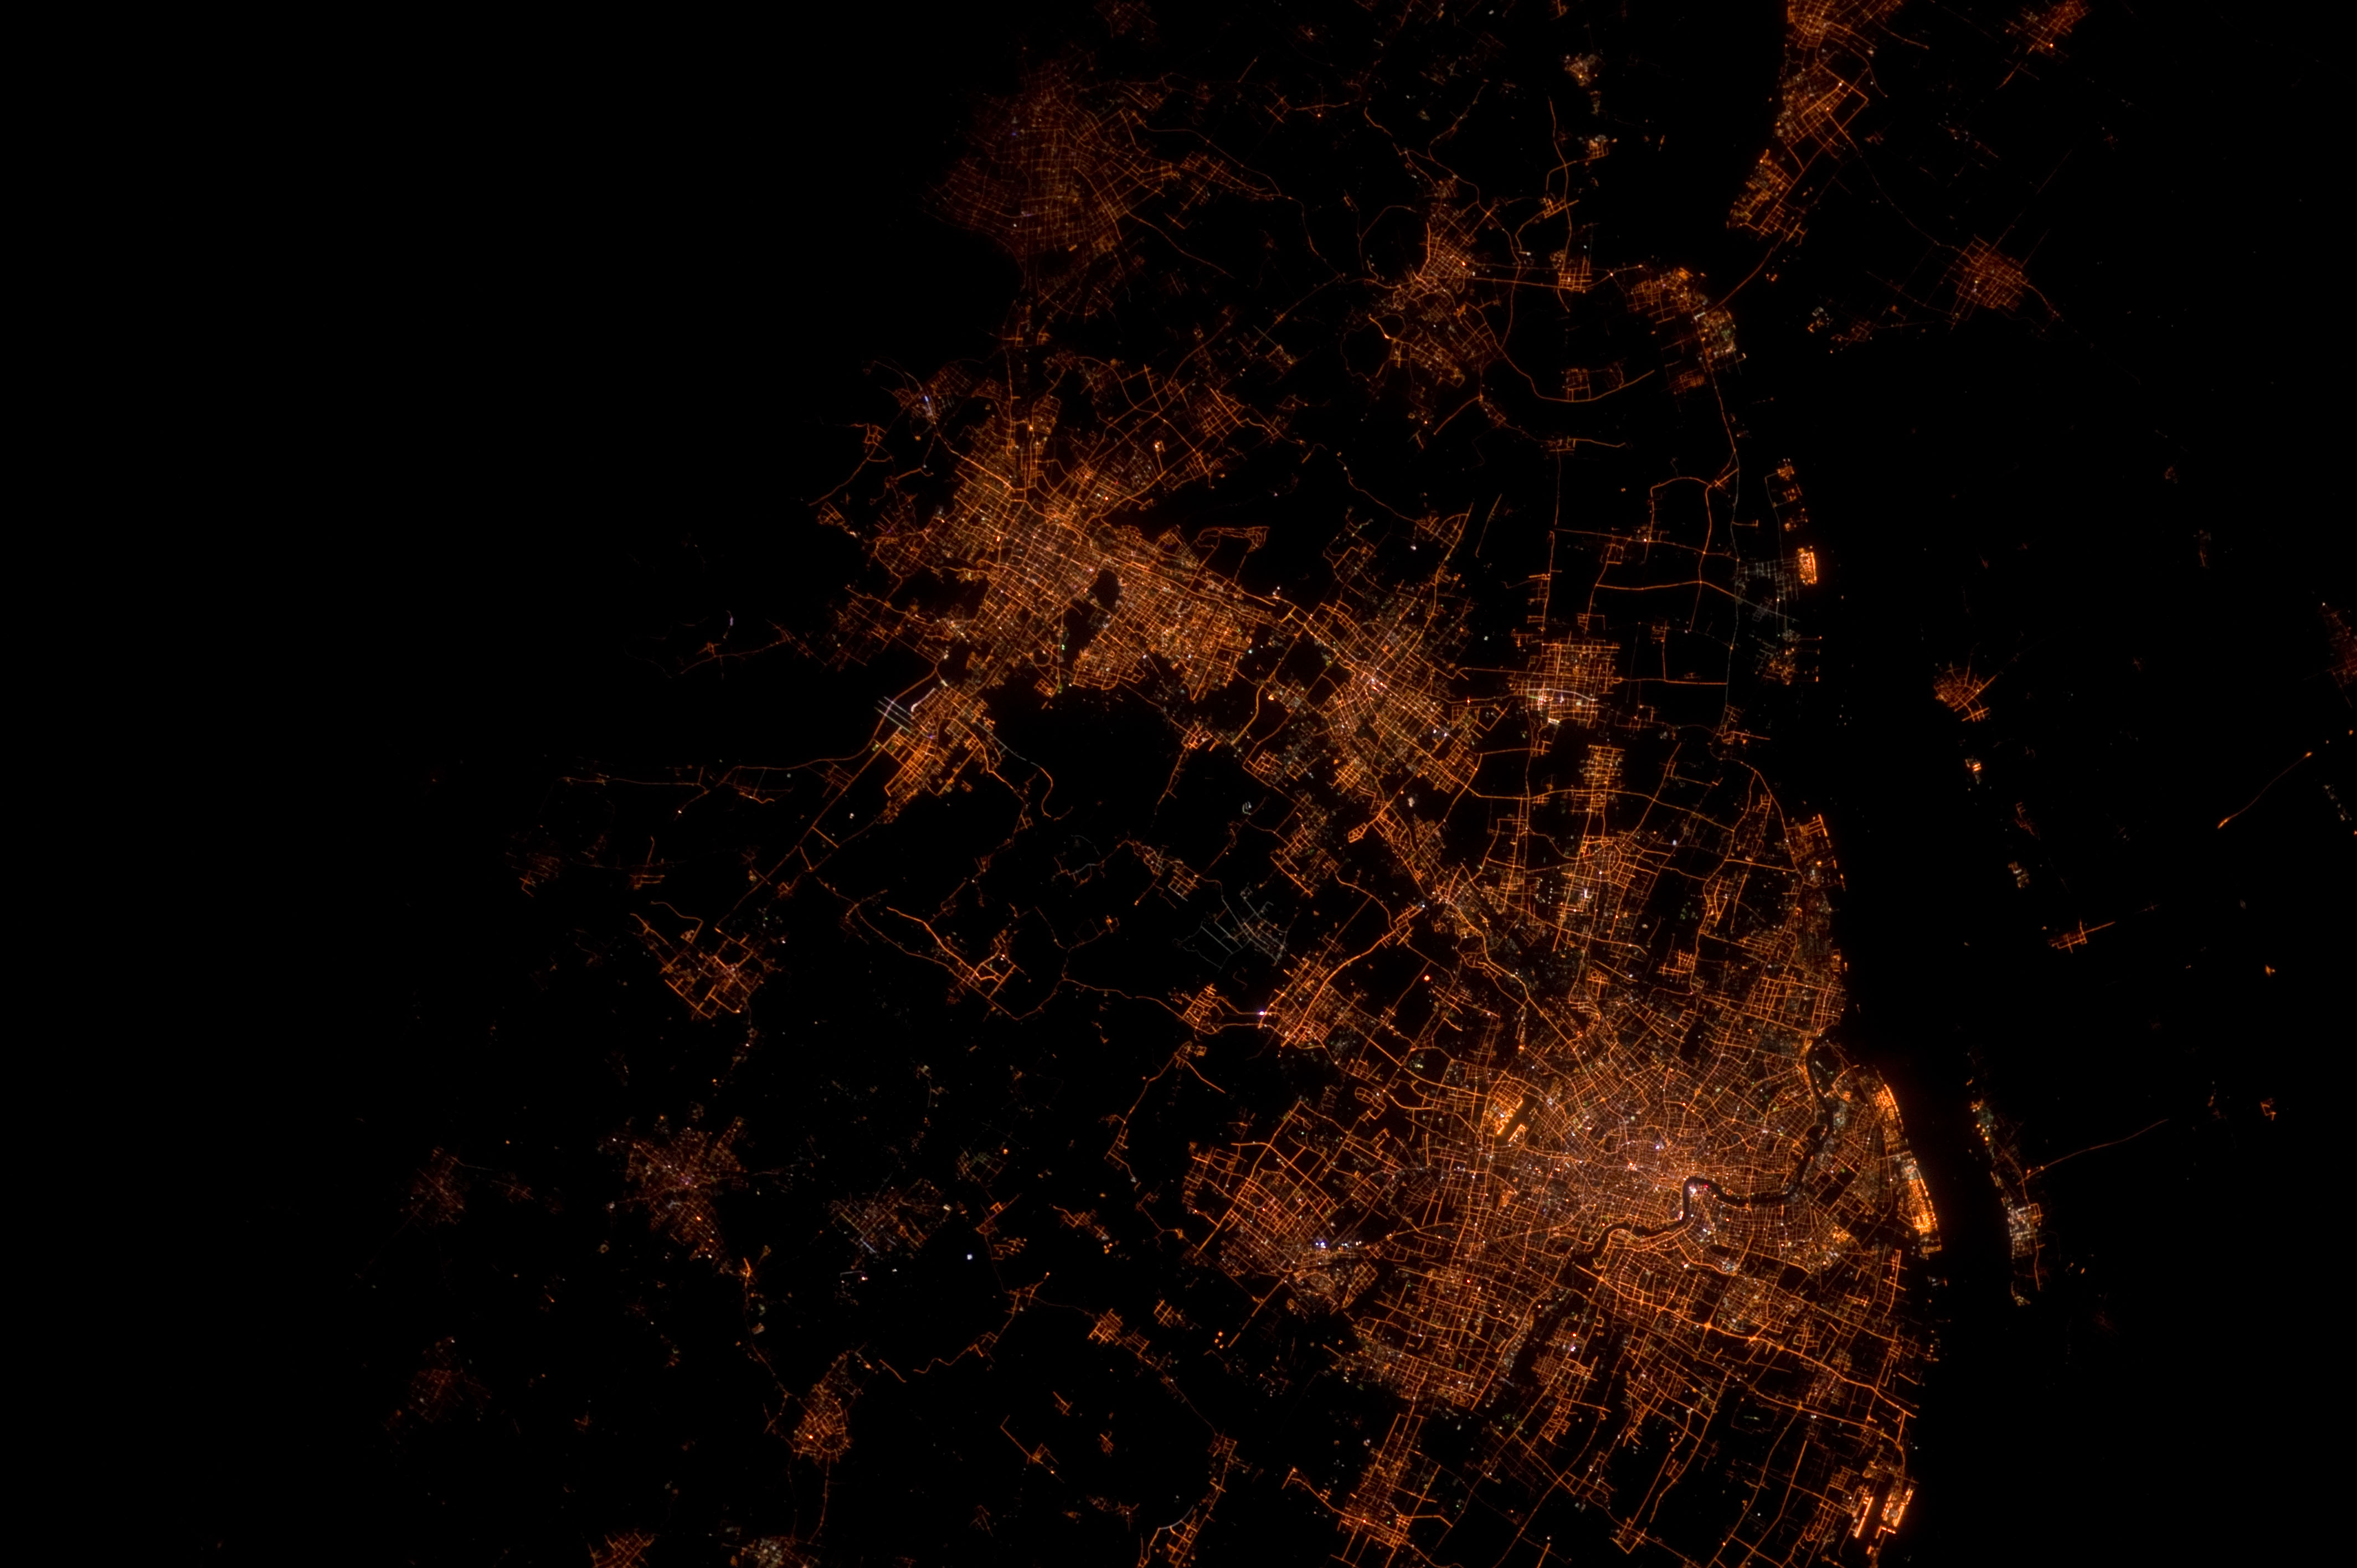
\includegraphics[width=1.5in]{images/4_01-ISS-30_Nighttime_view_of_Shanghai.jpg}
\caption{国际空间站拍摄的城市夜景(图片来自于维基共享资源计划)}
\end{figure}

可以说,太阳的光和热深深的渗透到我们文化的底层。在我们的大多数文化里,东、西、南、北四个方位是在儿童时期便教育给下一代的基本概念,我们会借助于太阳东升西落或者房屋、街道的布局来表达它们。然而,仔细考究四方的严格定义,必须得对日月星辰的运行有透彻的理解才可以。而因为这些基本概念潜入、物化在我们文化的各处,就像鱼儿不知道水的存在,我们也往往忘记了这些基本概念的来源。瓦克星则给我们一个反思的机会。

当我从新思考瓦克星环境里的四方概念时,走了一段弯路,才意识到四方概念的本质。

东、西:地球上是太阳在春秋分东升西落的方位;然而瓦克星的春秋分的时间如何精确测定?
南:正午的太阳位置、立杆影子最短、太阳的光强最大的位置;然而有两个太阳,如何处理?
北:地球是北极星的位置;然而如果瓦克星没有北极星,那怎么测北?

似乎确定每个方向都会遇到一些问题。

我从南开始入手,写了数值模拟程序,看温带房子哪个方位布局才能最大获得阳光。我希望能看到一个不一样的结果,然而结果就是和地球一样的正南方。

由此,我才恍然大悟:自转轴相对保持恒定,这是四方概念成立的根源;所以,“北”是本质性的,其他三个概念都可以导出。

当然,瓦克星上还是有和地球不一样的地方。

比如,和四方联系的分至四时,在地球上会和昼夜平分、极昼、极夜现象联系起来。我们考察瓦克星时发现了一个奇特现象—双极昼现象。

\begin{figure}[ht]
\centering
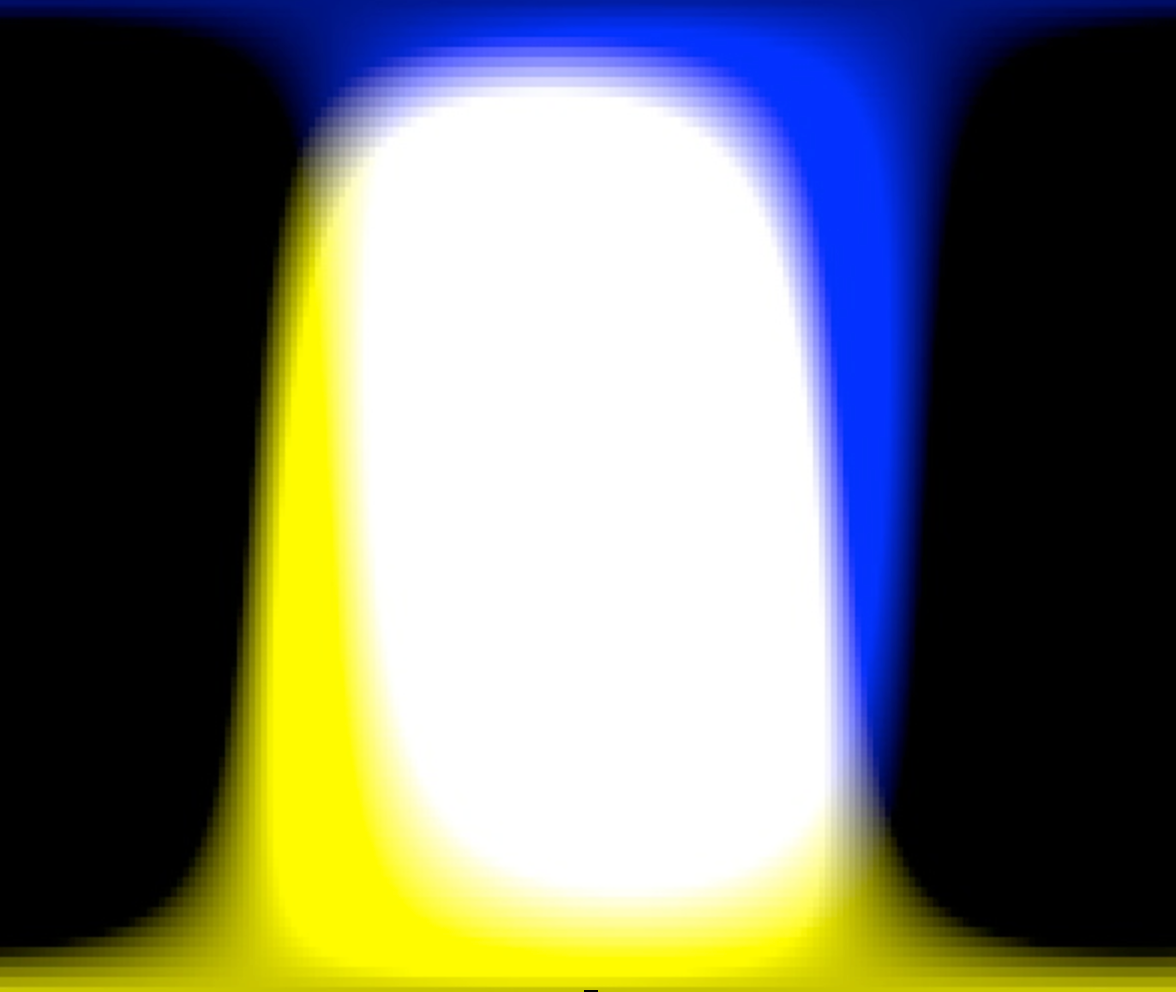
\includegraphics[width=1.5in]{images/4_02-day-night.png}
\caption{瓦克星上的双极昼现象}
\end{figure}

我们可以清楚看到,瓦克星南北两极都处于极昼。

\subsection{昼夜晨昏}

\subsection{年}

\subsection{季节}

\section{再造行星世界}

\subsection{大陆与海洋}

\subsection{温室效应}

\subsection{气温的纬度分布}

\subsection{大气环流}

\subsection{海气耦合}

\subsection{理想大陆}

\section{重建生物圈}

\subsection{异速生长律}

\subsection{植物形态}

\subsection{动物形态}

\subsection{演化}

\subsection{生态带}

\section{另辟蹊径的文明}

\subsection{数制}

大约在 18000 ~ 20000 BC 的 Ishango 骨刻,是目前人们发现的最早和数目有关的考古实物,它处在刻痕记事的阶段。
如果不考虑实物的形态,仅从抽象角度看,在这个阶段人们采用符号 1 的累记来表示更大的数目。
这种方式在表示形式上极为繁赘,尤其对大的数目,几乎不具有实际的可行性。但凭借这种简单的记号,人们有了对数目概念的理解。

\begin{figure}[ht]
\centering
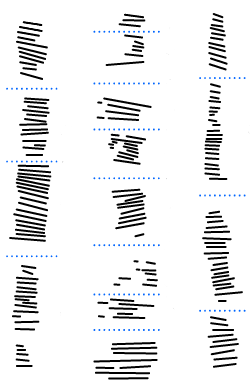
\includegraphics[width=1.5in]{images/IshangoAllColumns.png}
\caption{Ishango 骨刻(图片来自于维基共享资源计划)}
\end{figure}

在这个阶段,人们可以通过分堆的方法进行乘法运算。但这种方法仅仅限于小数目之间的乘法。

\begin{table}[tbhp]
\centering
\begin{tabular}{|c|c|c|c|c|}
\hline
\specialcell{ \ding{108} \\ \ding{108}\ding{108} } &
\specialcell{ \ding{108} \\ \ding{108}\ding{108} } &
\specialcell{ \ding{108} \\ \ding{108}\ding{108} } &
\specialcell{ \ding{108} \\ \ding{108}\ding{108} } &
\specialcell{ \ding{108} \\ \ding{108}\ding{108} } \\
\hline
\end{tabular}
\caption{计算 3 与 5 的乘积}
\end{table}

人类进入文明以后,有了对抽象符号更强的操作能力。在古埃及,人们发明了另外一种复杂的计数体系,它能表示整数、分数和相关运算。
我们这里仅仅简单展示整数的表示和乘法运算。

\begin{table}[tbhp]
\centering
\begin{tabular}{|c|ccccccc|}
\hline
数值 & 一 & 十 & 百 & 千 & 万 & 十万 & 百万 \\
符号 & \pmglyph{\Hone} & \pmglyph{\Hten} & \pmglyph{\Hhundred} & \pmglyph{\Hthousand} & \pmglyph{\HXthousand} & \pmglyph{\HCthousand} & \pmglyph{\Hmillion} \\
描述 & 单竖线 & 踵骨 & 绳圈 & 水莲 & 屈指 & 蝌蚪 & Heh 神\\
\hline
\end{tabular}
\caption{古埃及象形文字里的整数符号}
\end{table}

组合上述的基本符号,古埃及人可以表达一些相对较大的整数。但古埃及人组合这些符号的方式,并没有非常严格的方法:
既可以从左向右,也可以从右向左,有时也会竖写。除此以外,古埃及人做乘法的方式,更加显示出他们的数制还处于一种早期形态。
下图展示了古埃及人如何计算 11 与 35 乘积的过程。

\begin{figure}[ht]
\centering
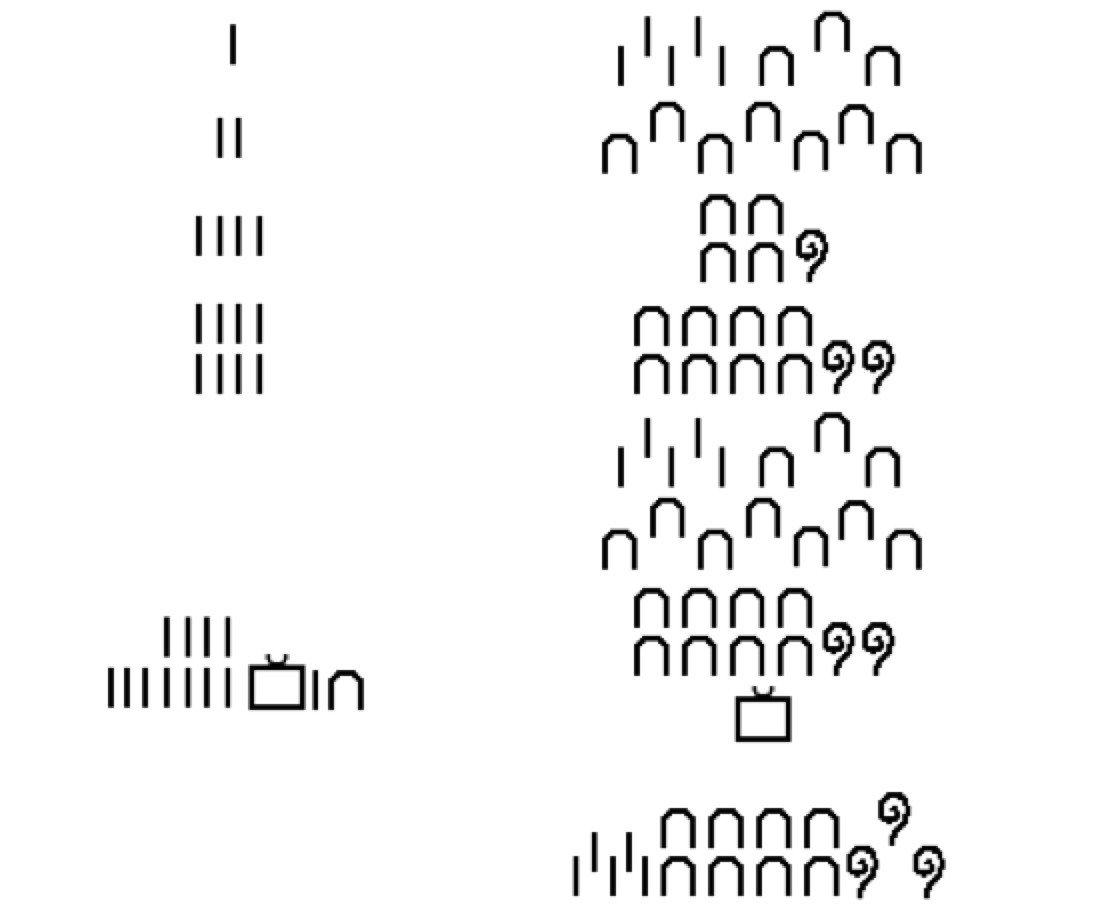
\includegraphics[width=3.5in]{images/ancient_egypt_multiplication.jpg}
\caption{计算 11 与 35 乘积}
\end{figure}

在这种方法里,首先构造 2 的幂的序列1、2、4、8……,同时 35 也按照 2 倍的关系相应扩大。
然后可以看出,11 能被分解成为了 1、2、8 的和,所以只要把 35 倍数里的 35、70、280 累加就可以得到结果。

但是数制的更加成熟的形态是数位制。在许多古文明中,数位制都被发明出来,如古巴比伦的 60 进制系统、古印第安文明的 20 进制系统。
对于乘法运算,中国古代很早就发明了九九乘法表,清华简中的“算表”作为考古实物依据,把发明年代至少向前推进到战国时代。
十进数位制和九九乘法表结合在一起,人们能够完整的表达所有自然数,并计算任意自然数的乘法。
当今,阿拉伯数字符号、十进数位制、九九乘法表都作为基础教育的内容,成为全人类分享的文明成果。

\begin{table}[tbhp]
\centering
\begin{tabular}{cccccccccccccccccccccccccccccccccccc}
  &   &   &   &   &   &   &   & 2 & 3 & 9 & 5 & 8 & 2 & 3 & 3\\
× &   &   &   &   &   &   &   &   &   &   &   & 5 & 8 & 3 & 0\\
\hline
  &   &   &   &   &   &   &   & 0 & 0 & 0 & 0 & 0 & 0 & 0 & 0\\
  &   &   &   &   &   &   & 7 & 1 & 8 & 7 & 4 & 6 & 9 & 9 &  \\
  &   &   &   &   & 1 & 9 & 1 & 6 & 6 & 5 & 8 & 6 & 4 &   &  \\
  &   & + &   & 1 & 1 & 9 & 7 & 9 & 1 & 1 & 6 & 5 &   &   &  \\
\hline
  &   &   &   & 1 & 3 & 9 & 6 & 7 & 6 & 4 & 9 & 8 & 3 & 9 & 0\\
\end{tabular}
\caption{竖式乘法的例子}
\end{table}

\subsection{逻辑}

\subsection{文字}

\section{余论}

\end{document}
